%\documentclass{amsart}

\documentclass{article}
\usepackage[letterpaper,hmargin=20mm,vmargin=20mm]{geometry}
\usepackage[nosetup, colorlinks]{tony}
\usepackage{graphicx}

\usepackage{amsmath,amssymb}
\usepackage{siunitx}

\usepackage{mathpazo}
\usepackage{microtype}
\usepackage{multicol}

\usepackage{diagbox}

\usepackage{color}
\usepackage[dvipsnames]{xcolor}
%\usepackage[printwatermark]{xwatermark}
%\newwatermark*[allpages,color=gray!50,angle=45,scale=3,xpos=0,ypos=0]{DRAFT}

\usepackage{tikz}
\usetikzlibrary{arrows}

\DeclareMathOperator{\sgn}{sgn}
\DeclareMathOperator{\NLL}{NLL}
\newcommand{\sind}[1]{^{(#1)}}

\title{Prediction of airline departure delays}
\author{Tony Zhang and Menghua Wu}
\date{December 16, 2016}

\begin{document}
\maketitle

\begin{multicols}{2}

% % % % % % % % % %
%    INTRODUCTION
% % % % % % % % % %

\section{Introduction}

Often, people purchase plane tickets
to minimize monetary cost.
However, price is not the only consideration
when consumers purchase tickets---
not all flights are created equal.
In particular,
flyers often care about and take into account
the risk that a flight will be delayed.
This paper hopes to quantify this risk
on the basis of past flight delay data.

The United States Bureau of Transportation Statistics (BTS)
compiles comprehensive datasets annually
regarding the nation's transportation infrastructure,
including aviation, maritime, highway, and rail.
In this paper, we focus on the aviation dataset,
which reports on a wide range of variables concerning individual flights,
including carrier, origin and destination, and flight delays.
We will primarily concern ourselves with classification:
whether a flight is delayed or not.

% TODO change this section?
We downloaded data from June 2015 to May 2016, inclusive.
Each month of data reports on
approximately 500000 individual flights.
Notably, some of the data is missing.
We used these data to build a classifier
that predicts whether or not a flight's departure
is expected to be delayed.
We combined several methods of classification
and compare their results here.


\section{Data preprocessing}

% TODO describe this

For simplicity,
we only considered the following data features:
\begin{itemize}
    \item
    Departure date and time
    \item
    Airline
    \item
    Origin and destination airports
\end{itemize}

Since airline and airports are categorical features,
we encoded them as one-hot vectors.
In the data subset we considered,
there were 14 airlines and roughly 250 airports.

For date and time,
we began by encoding them as days into a year
and minutes into the day.
This representation leaves much to be desired, however.


\subsection{Cyclic features}

Features such as time of day and day of year
are naturally cyclic.
Representing them on a linear scale
therefore imposes an unnatural metric on them.
For instance,
if we naively represent times as ``minutes into day",
the time 23:59 will be considered ``more similar"
by any machine learning model to noon than to 00:01,
which disagrees with our intuitive notions of closeness.

A better representation of cyclic data
would respects our notions of closeness.
An obvious choice is to map a linear data point $x \in [0, T)$
onto a unit circle by
\begin{equation}
    \label{eq:cyc-mapping}
    x \mapsto \lt(\cos\f{2\pi x}{T}, \sin\f{2\pi x}{T}\rt).
\end{equation}
For instance, if we were to encode the time of day,
noon would have ``angle" $\f{2\pi x}{T} = \pi$
and would thus get mapped to the point $(-1, 0)$.

We encoded dates (with $T$ being a year)
and time (with $T$ being a single day).
In preliminary testing,
we found that this encoding
noticeably improved classification accuracies
for a variety of models,
including logistic regression and random forests.

\subsection{Dataset partitioning}

% TODO

\section{Logistic regression}

To establish a baseline accuracy
and to benchmark our future efforts,
we began with a regularized logistic regression classifier
with $L_2$ regularization.
Recall that such a classifier attempts to minimize a loss of the form
\begin{equation}
    \label{eq:log-reg-l2-loss}
    J(w, b) = \f12 w^T w + C \sum_i \log\lt(1 + e^{-y\sind{i}(w^T x\sind{i} + b)}\rt)
\end{equation}
where the sum is taken over all training data points.
The parameter $C$ controls the amount of regularization;
a smaller value of $C$ produces greater regularization.

We performed a sweep over log-uniformly spaced $C$
from $10^{-5}$ to $10^5$ (with factors of 10 between each $C$).
Optimizing for validation accuracy,
we selected $C^* = 100$,
which yielded a test accuracy of $0.661$.

Unsurprisingly,
replacing the first term in Equation~\ref{eq:log-reg-l2-loss}
with an $L_1$ norm on $w$
gives us the loss function for a classifier with $L_1$ regularization.
Performing a sweep over $C$ as we did previously
and optimizing for validation accuracy again,
we found an almost identical test accuracy of $0.660$.

We present the validation accuracies
under both regularization schemes
for the values of $C$ we tested
in Figure~\ref{fig:log-reg-c-sweep}.

\begin{figure*}[t] %  figure placement: here, top, bottom, or page
   \centering
   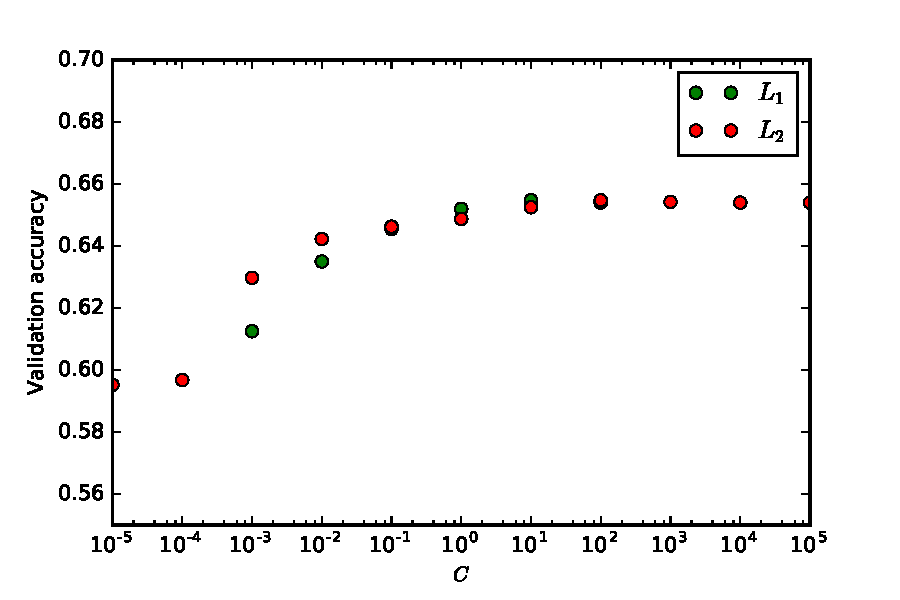
\includegraphics[width=4in]{img/log-reg-C-sweep.pdf}
   \caption{Logistic regression validation accuracies
   under $L_1$ and $L_2$ regularization
   for varying values of regularization parameter $C$.}
   \label{fig:log-reg-c-sweep}
\end{figure*}

\section{Multilayer perceptrons}

We next attempted to improve upon our previous results
with multilayer perceptrons:
vanilla neural networks.
We minimized mean cross-entropy loss with the Adam optimizer,
computing gradients by backpropagation.
Recall that cross-entropy loss for a single data point $x\sind{i}, y\sind{i}$
is given by
\begin{equation}
    J\sind{i}(w) = -y\sind{i}\log\hat y\sind{i} - (1-y\sind{i})\log(1-\hat y\sind{i})
\end{equation}
where $y\sind{i}$ is a binary training label (either 0 or 1)
and where $\hat y\sind{i}$ is the probability estimate from the network.

We also imposed $L_2$ regularization on the network weights,
governed by regularization parameter $\alpha$,
such that the training loss function is given by
\begin{equation}
    J(w) = \f12\alpha w^T w + \sum_i J\sind{i}(w).
\end{equation}

We experimented with various architectures, activations, and $\alpha$.
Given the large space of possible hyperparameter combinations,
it was infeasible to find a best set of hyperparameters exhaustively.
As such,
we explored the effects of each hyperparameter
by holding values of the others fixed.

\subsection{Architecture}

In experimenting with network architecture,
we fixed $\alpha = 10^{-5}$.
We began by exploring different numbers of hidden layers,
finding that deeper networks provided no significant improvement
over single-hidden-layer networks.
Thus, we restricted our attention
to networks with just a single hidden layer.

We show our findings in Figure~\ref{fig:mlp-plots}
for three different activation functions on the hidden nodes;
it's apparent that varying the number of hidden nodes
did not provide any substantive improvement in our results.

\begin{figure*}[t] %  figure placement: here, top, bottom, or page
   \centering
   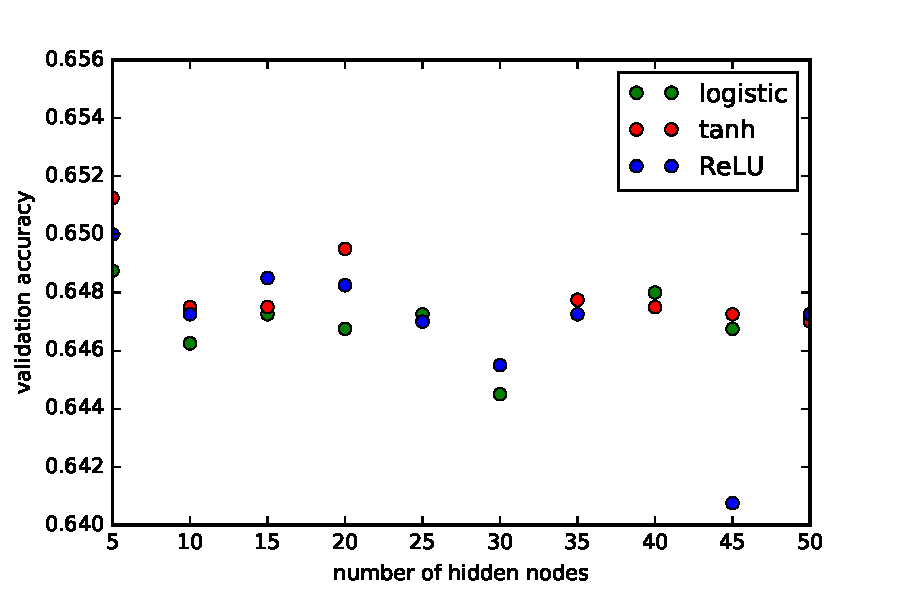
\includegraphics[width=3in]{img/mlp-one-hidden-layer.pdf}
   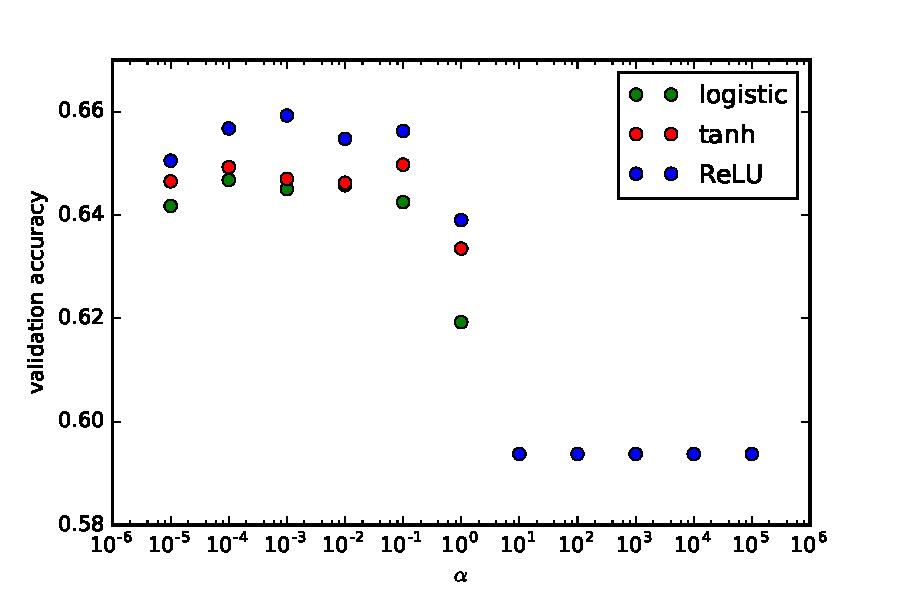
\includegraphics[width=3in]{img/mlp-alpha-experiment.pdf}
   \caption{Single-layer multilayer perceptron validation accuracies.
   The plot on the left shows the results of varying the number of hidden nodes
   while fixing $\alpha = 10^{-5}$.
   On the right, we fixed the size of the hidden layer at 25 nodes
   and varied $\alpha$.}
   \label{fig:mlp-plots}
\end{figure*}


\subsection{Regularization}




% TODO RESULTS

\section{Random forest classification}

We turned to ensemble methods 

We leveraged existing random forest implementations
and determined the optimal parameters for classifying our data.
We determined the best model using our validation data
and tested on our testing data.
%There may be strong relationships between
%month of year and airline delay,
%as the holiday season is often associated with
%inclement weather and an increase in delays.
%Therefore, we trained a separate random forest classifier
%for each month, in additional to a single classifier
%for the combined data.
%For each month,
%the resultant model was an average of
%that month's classifier and the combined classifier,
%weighted by validation error.
%On the testing data,
%the combined classifier performed better
%than each classifier alone,
%perhaps due to increased generalization.

The following sections explore the effects of varying hyperparameters,
with all else held equal.
Default values are bootstrapped samples,
10 estimators, an early stopping impurity threshold of $10^{-7}$,
and no maximum tree depth,
feature masking, or warm start.

\subsection{Bootstrapping}

Bootstrapping allows us to sample with replacement
from the dataset,
emulating sampling from the general population.
When we sample without replacement instead,
training accuracy increased,
but validation accuracy decreased,
potentially due to overfitting on more sample points during training.

% bootstrap
%Training data score 0.9757875
%Testing data score 0.6527087149960743
%
% no bootstrap
%Training data score 0.9998625
%Testing data score 0.6186862077990055
\begin{center}
    \begin{tabular}{c| c c}
        method & bootstrap & no bootstrap \\
        training acc
        		& 0.976 & 0.999 \\
        validation acc
        		& 0.653 & 0.619
    \end{tabular}
\end{center}

\subsection{Number of estimators}

Random forest contains bagged trees,
so by changing the number of estimators,
we can control overfitting and improve prediction accuracy.
Increasing the number of trees
improved both training and validation accuracy.
However, since training more estimators
is computationally intensive,
we did not train more than 32 trees.
%n_estimators 2
%Training data score 0.9739375
%Testing data score 0.6351740382098927
%
%n_estimators 8
%Training data score 0.9671375
%Testing data score 0.6430253860246009
%
%n_estimators 16
%Training data score 0.9887
%Testing data score 0.6517927244176916
%
%n_estimators 32
%Training data score 0.9971375
%Testing data score 0.6585972258571055
\begin{center}
    \begin{tabular}{c|c c c c}
        $n$ trees
        		& 2 & 8 & 16 & 32 \\
        training acc
        		& 0.974 & 0.967 & 0.989 & 0.997\\
        validation acc
        		& 0.635 & 0.643 & 0.651 & 0.658
    \end{tabular}
\end{center}

\subsection{Maximum tree depth}

By default, tree depth is unconstrained,
so the classifier runs until all nodes
are expanded into valid leaves.
We experimented with imposing a maximum depth
as a form of early stopping.
This method generally decreased training accuracy,
but increased validation accuracy
for some depths.
%max_depth_leaf 4
%Training data score 0.6570625
%Testing data score 0.6447265113844544
%
%max_depth_leaf 8
%Training data score 0.679025
%Testing data score 0.6563726773096048
%
%max_depth_leaf 16
%Training data score 0.75025
%Testing data score 0.6665794294687255
%
%max_depth_leaf 32
%Training data score 0.8992
%Testing data score 0.6656634388903429
%
%max_depth_leaf 64
%Training data score 0.9726625
%Testing data score 0.6540172729651924
%
%max_depth_leaf 256
%Training data score 0.976025
%Testing data score 0.6472127715257786
\begin{center}
    \begin{tabular}{c|ccccc}
        max depth &
          4 & 8 & 16 & 32 & 256 \\\hline
        training acc. &
          0.657 & 0.679 & 0.750 & 0.899 & 0.976\\
        validation acc. &
          0.644 & 0.656 & 0.667 & 0.654 & 0.647
    \end{tabular}
\end{center}
Imposing a maximum tree depth effectively
reduces overfitting to training data.

\subsection{Masking features}

When building each tree,
we can ignore a subset of features
when looking for the best split.
However, masking a percentage of features
did not significantly affect training or
validation accuracy.
This may be due to the sparsity
of our data, with many one-hot vectors.

\subsection{Early stopping}

If we do not constrain the depth of the tree,
an alternative method of early stopping
is to increase the maximum size of each leaf.
However, changing this value (up and down)
was not as effective as
limiting tree depth, and had little effect.

\subsection{Warm start}

For each estimator,
we can either train a new tree from scratch (default),
or use the results of the previous run
as a starting point (warm start).
Warm start had little effect.

\subsection{Optimal model}

Using our validation data,
we selected the best model
of 32 estimators, a max depth of 16,
and default values for all other parameters.
We obtained a testing accuracy of 0.687\%,
which is a slight improvement on logistic regression.

\section{Dataset transformations}
\label{sec:dataset}

The raw dataset from the BTS
includes unconventional features,
so we preprocessed our dataset
to improve classification feasibility.

Use best parameters from previous section.

\subsection{Geographic relations within data}

So far, we have considered origin and destination data
as discrete values,
each airport with an equal probability of causing delays.
That is, the distance between any two airports
(as one-hot vectors) is the same.
However, this may not be the case in the real world.

\subsection{Geographic displacement}

East west vs. vice versa, etc.

\section{Comparison with other methods}

We compared our ensemble classifier
with other types of classifiers,
including logistic regression, a neural network,
and a kernelized Pegasos classifier
with the Gaussian RBF kernel.
Due to the large size of our dataset,
we were limited to
stochastic and minibatch methods.

\section{Conclusions}

xxx

\end{multicols}

\end{document}

